\documentclass{css}
%\documentclass[english]{css}

\usepackage[dvips]{graphicx}
\usepackage{latexsym}

\def\|{\verb|}

\newcommand{\cssyear}[0]{2023}
\newcommand{\cssname}[0]{CSS 2023}
\newcommand{\cssversion}[0]{2023/06/01}
\newcommand{\cssemail}[0]{css2023-office@iwsec.org}

\begin{document}

%% 本文が和文の場合,タイトル・著者名・著者所属・概要は,和文・英文共に必須.
%% If you prepare this manuscript in English, there is no need to put Japanese metadata (title, author names, affiliations, abstract, and keywords) in it.

\title{Isolation Forestを用いた\\IoT向け異常検知手法に関する考察}
\etitle{A Study on Anomaly Detection Method \\for IoT using Isolation Forest}

\affiliate{XX}{東京工業大学 情報理工学院 数理・計算科学系\\
Department of Mathematical and Computing Sciences, School of Computing, Tokyo Institute of Technology}
\affiliate{YY}{株式会社YYセキュリティ研究所\\
Security Laboratories, YY Corporation}
\paffiliate{ZZ}{国立研究開発法人ZZ研究所\\
National Institute of ZZ}

%% メールアドレスは省略可能だが,代表者のメールアドレスは必須.
%% 姓名の間は半角スペースを入れること.

\author{菅田 大輔}{Daisuke Sugata}{XX}[sugata.d.aa@m.titech.ac.jp]
\author{安全 花子}{Hanako Anzen}{XX, YY, ZZ}

%% the following is author command for english option.
%% at least one e-mail address is required.

%\author{Taro Joho}{XX}[taro.joho@xx.ac.jp]
%\author{Hanako Anzen}{XX, YY, ZZ}

\begin{abstract}
    本論文では、Isolation Forestを用いたIoT向け異常検知手法の改善を行なった。この研究の背景に、IoT(Internet of Things)の普及がある。実際、2030年には約300億台ものデバイスが利用されると予測されており、すべてのIoT機器のセキュリティ確保が重要な課題となっている。特に2016年のMirai型マルウェアによるDDoS攻撃はその必要性を浮き彫りにした。今回は、専門的なセキュリティ対策が難しい家庭内ネットワークなどの小規模環境に着目し、軽量で高速な異常検知システムの提案を目指した。Isolation Forestは軽量で高速に動作する異常検知手法として注目されているが、これを用いた従来の方法には二つの問題が存在する。閾値を手動で設定する必要がある点と、異常判定のアルゴリズムの精度に限界がある点である。これらの課題を解決するために、本研究ではロジスティック回帰を用いた判定アルゴリズムを提案する。提案手法を二つのデータセットで実験した結果、精度がそれぞれ84.4\%から91.1\%、84.6\%から94.5\%に改善したことを確認した。

\end{abstract}

%% キーワード (1--5単語) の記載は任意.

\begin{jkeyword}
Isolation Forest, IoT, IDS, 異常検知
\end{jkeyword}

\begin{eabstract}
abstract

\end{eabstract}

%% the following keyword part is optional and can be omitted.

\begin{ekeyword}
Isolation Forest, IoT, IDS, Anomaly Detection
\end{ekeyword}

%% if you use english opsion, you should put your English abstract in the abstract environment.
%% eabstract is not displayed in english mode.

\maketitle

%1
\section{はじめに}

\section{研究方法}

\subsection{Isolation Forestの説明}
Isolation Forest(以下,iForest)は,外れ値検出のためのアルゴリズムである。iForestは異常データが少数であり、離れているという前提に基づいている。ランダムにデータを分割していくと、異常データは相対的に早く分離される。iForestは以下のステップで実行される。

\subsubsection*{1. データの分割}
ランダムに選んだ特徴量から、ランダムに選んだ値をもとにデータを分割する。これを一定回数繰り返し、複数のツリーを作成する。

\subsubsection*{2. 異常スコアの算出}
データがツリーの枝に到達するまでの平均パスをもとに、異常スコアを算出する。具体的な計算式は以下の通りである。

ここで、$E(h(x))$はデータ点$x$の平均パス長、$c(n)$はデータセットのサイズ$n$に依存する定数である。

\subsubsection*{3. 異常判定}
先ほど計算した異常スコアをもとに異常検知を行う。通常、トレーニングデータの異常スコアの上位10\%を閾値として設定し、それを超えたデータを異常と判定する。


\subsection{IDSの概要}
本研究では、小規模なIoT環境に適したIntrusion Detection System(IDS)の設計について検討する。具体的には、Isolation Forestを用いた異常検知手法が提案され、その有効性を評価する。

\subsection{全体の設計}
IDSの設計は以下の3つのセクションに分けられる:
\begin{enumerate}
    \item \textbf{データの前処理}:
        \begin{itemize}
            \item 入力データを適切な形式に変換する。
            \item 不必要な特徴量の削除やデータの標準化、ラベルエンコーディングを行う。
        \end{itemize}
    \item \textbf{特徴量選択}:
        \begin{itemize}
            \item 判定に重要な特徴量を選択し、過学習を防ぎ、検知精度を向上させる。
            \item Random Forestを用いて特徴量の重要度を算出し、重要な特徴量を選択する。
        \end{itemize}
    \item \textbf{攻撃の判定}:
        \begin{itemize}
            \item iforestを用いて通信が攻撃通信であるかを判定する。
            \item 特徴量の選択後、Isolation Forestで異常検知を行う。
        \end{itemize}
\end{enumerate}

\subsection{実装}
実装は以下のステップで行う:
\begin{enumerate}
    \item \textbf{データの前処理}:
        \begin{itemize}
            \item はじめに、不必要な特徴量の削除を行う。(データの標準化を行う必要なし?)Iforestに入力できるのは数値データだけなので、カテゴリカルデータを数値データに変換する。one-hotエンコーディングを用いてラベルのエンコーディングを行う。
        \end{itemize}
    \item \textbf{特徴量選択}:
        \begin{itemize}
            \item Random Forestを用いて特徴量の重要度を算出する。その後、重要度をもとに上位1割の特徴量を使用する。
        \end{itemize}
    \item \textbf{攻撃の判定}:
        \begin{itemize}
            \item 攻撃通信、正常通信のそれぞれでトレーニングされたサブシステムが、Isolation Forestによって異常検知を行う。
            \item それぞれのサブシステムの結果を2通りで組み合わせ、最終的な判定を行う。
        \end{itemize}
\end{enumerate}


\section{iForestの問題点の整理}
Isolation Forestを異常検知手法として使用する際,どのような問題があるのかを明らかにするため,事前実験を行った.はじめにデモデータを使用して,iForestの挙動を確認した.その考察をもとに、特徴量選択手法の提案を行なった

使用したデモデータは、(2.5, 2.5)と(-2.5, -2.5)を中心とした
正常データ群と、10から-10の範囲に一様に分布した異常データ群からなる.二次元の場合のデモデータを図\ref{fig:demodata}に示す.

\begin{figure}[tb]
    \centering
    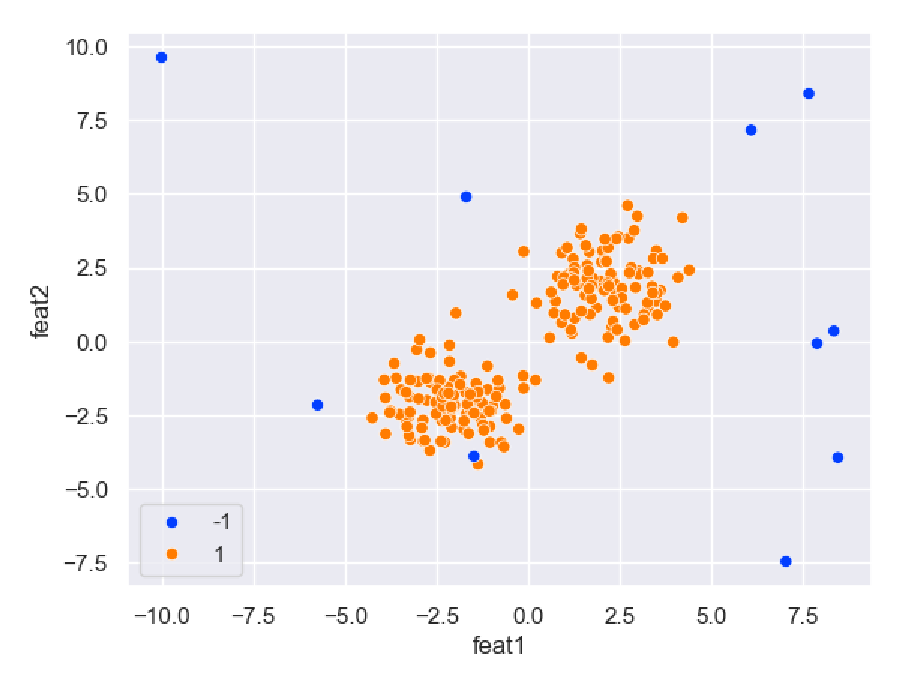
\includegraphics[width=\linewidth]{pictures/eps/demodata.eps}
    \caption{デモデータに関する図の説明(和文)}
    \ecaption{Description of the dim\_vs\_accu figure (English).}
    \label{fig:demodata}
\end{figure}

はじめに、デモデータと特徴量数の関係を調査した.図\ref{fig:dim_vs_accu}に示すように、特徴量数が増えるにつれて、異常検知の精度が単調に向上することがわかった.また、精度ののびは増加に反比例して緩やかになっていることもわかる。ゆえに、iForestは目標とする精度に対して十分な特徴量数が存在すると言える。

\begin{figure}[tb]
    \centering
    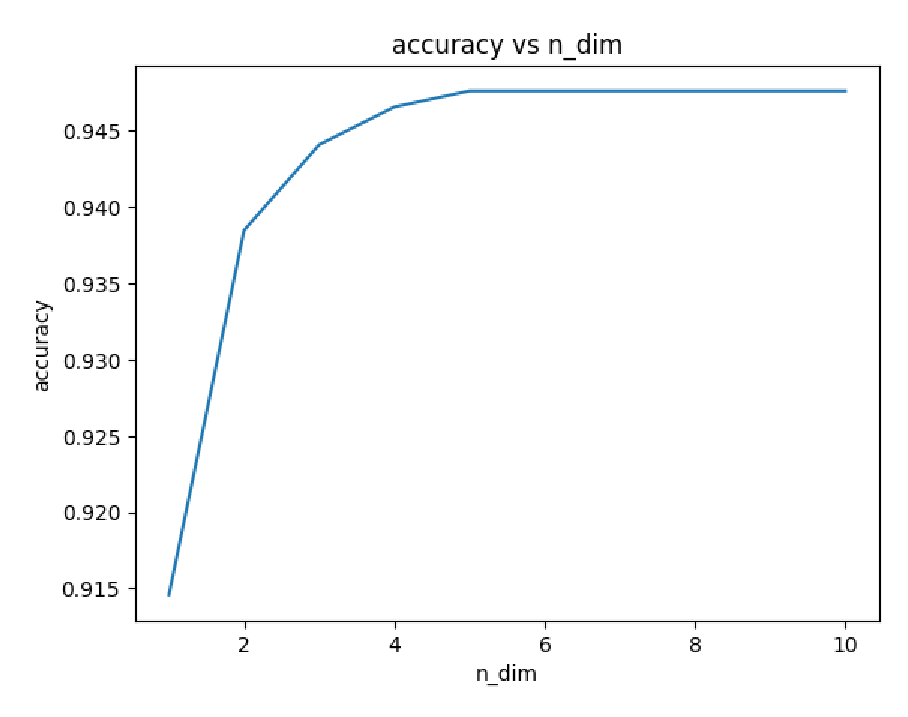
\includegraphics[width=\linewidth]{pictures/eps/dim_vs_accu.eps}
    \caption{dim\_vs\_accuに関する図の説明(和文)}
    \ecaption{Description of the dim\_vs\_accu figure (English).}
    \label{fig:dim_vs_accu}
\end{figure}

パケット通信を監視して得られたデータセットの全ての特徴が、異常検知に有効であるわけではない。iForestは特徴量同士の重みづけを行わないため、判定に有効でない特徴量が混ざると精度が低下すると考えられる。そこで、図\ref{fig:noise_accu}に示すように、ノイズとなる特徴量を混ぜた時の精度を調査した。この結果から、ノイズとなる特徴量が混ざると精度が低下することがわかった。また、今回の実験の場合だと、ノイズとなる特徴量が判定に有効な特徴量数の2倍以上になると、精度が急激に低下することがわかった。

\begin{figure}[tb]
    \centering
    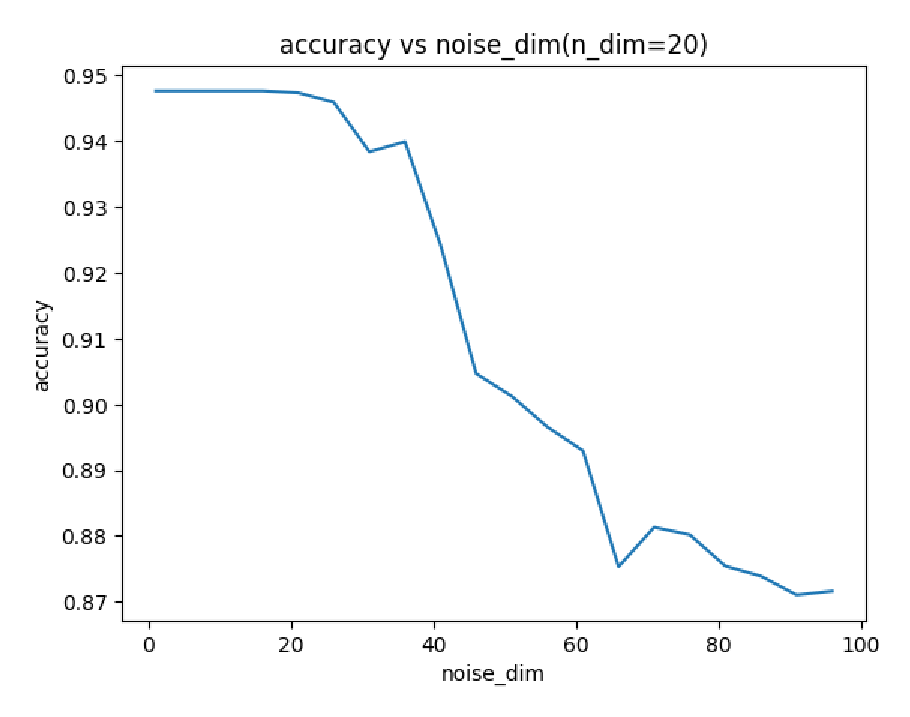
\includegraphics[width=\linewidth]{pictures/eps/noise_accu.eps}
    \caption{noise\_accuに関する図の説明(和文)}
    \ecaption{Description of the noise\_accu figure (English).}
    \label{fig:noise_accu}
\end{figure}

前の実験から、データセットからノイズとなる特徴量を取り除くことが重要であることがわかった。ところで、iForestはツリーベースの異常検知手法である。そこで、同じくツリーベースのRandam Forestから特徴の重要度を算出すれば、ノイズとなる特徴量を取り除けるのではないかと考えた。図\ref{fig:select_noise}は、Random Forestで算出した特徴量の重要度を表している。このグラフは、ノイズ特徴量を判別できていることがわかる。そして、実際にノイズ特徴量を取り除いた場合の精度を調査したところ、精度は???\%から0.945\%まで向上した。この結果から、Feature Importanceによる特徴量選択手法は精度の向上に有効ではないかと考えた。

\begin{figure}[tb]
    \centering
    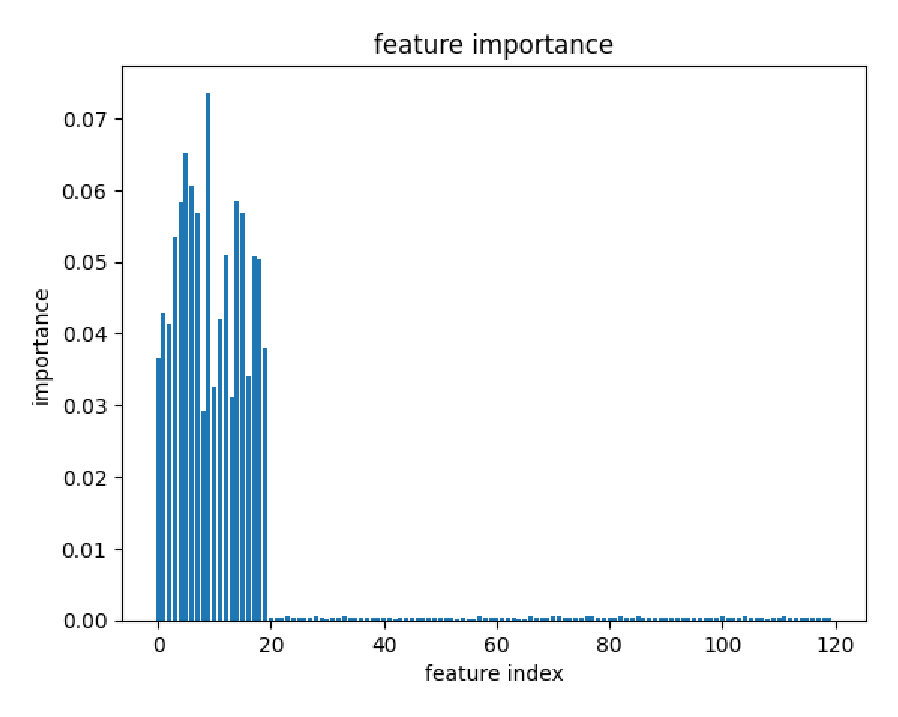
\includegraphics[width=\linewidth]{pictures/eps/select_noise.eps}
    \caption{select\_noiseに関する図の説明(和文)}
    \ecaption{Description of the select\_noise figure (English).}
    \label{fig:select_noise}
\end{figure}

\subsection{より効果的な判定の組み合わせ方について}
Iforestを用いた異常検知手法では、攻撃データと正常データのそれぞれでトレーニングされたサブシステムが、Isolation Forestによって異常検知を行う。最終的な判定は、これらの結果を組み合わせることで行う。AbuAlgahamらの研究では、表\ref{tab:combination}のようにそれぞの判定器の結果を組み合わせることで、最終的な判定を行なっている。
しかし、表\ref{tab:combination}のようにマッピングを行うことは2つの問題を抱えている。一つ目は、1. それぞれの判定器の異常スコアの閾値を適切に設定する必要があること, 2. 異常判定が、2つの異常スコアから直線的に決定されるため、異常スコアの分布によっては適切な判定ができないことである。

\begin{table}[tb]
    \caption{組み合わせアルゴリズム(和文)}
    \ecaption{combination algorithm (English).}
    \centering
    \footnotesize
    \begin{tabular}{lcc}
        \hline
        Normal subsystem & Attack subsystem & combination result\\
        \hline
        Normal & Anomaly & Normal \\
        Anomaly & Normal & Anomaly \\
        Normal & Normal & Anomaly \\
        Anomaly & Anomaly & unknown \\
        \hline
    \end{tabular}
    \label{tab:combination}
\end{table}

そこで、本研究では、異常スコアの分布によって適切な判定ができるように、異常スコアをロジスティック回帰を用いて判定する手法を提案する。この手法では、それぞれのサブシステムの異常スコアを入力とし、ロジスティック回帰によって異常判定を行う。この手法を用いることで、1.iForestの閾値を設定する必要がない 2. 閾値による直線的な分割よりも、より正確な分割が行える という利点がある。

\section{結果と考察}

\subsection{比較するアルゴリズム}

本研究では、以下の2つの比較を行った。
特徴量エンジニアリングの効果の比較を行うため、特徴量選択を行わなかった場合と、Random Forestを用いた特徴量選択手法を用いた場合の結果を比較する。また、判定の組み合わせアルゴリズムの比較には、2つのサブシステムの結果をマッピングする手法と、Rogistic Regressionを用いて判定を行う手法の結果を比較した。

\begin{enumerate}
    \item \textbf{特徴量エンジニアリングの比較}:
        \begin{itemize}
            \item 特徴量選択なし
            \item Random Forestを用いた特徴量選択手法
        \end{itemize}
    \item \textbf{判定の組み合わせアルゴリズムの比較}:
        \begin{itemize}
            \item マッピングして判定
            \item Rogistic Regressionを用いて判定
        \end{itemize}
\end{enumerate}

\subsubsection{実験環境}

実験はMac Book Pro 2017 2.3GHz Intel Core i5, 8GB RAMで行った。また、実験に用いたプログラムはPython3.10.4で実装した。Isolation ForestやRandom Forestの実装には、scikit-learnのライブラリを用いた。

\subsubsection{データセット}
本実験では、以下の2つのデータセットを用いた。

\begin{enumerate}
    \item \textbf{NSL-KDD}:
        KDDCUP99の問題点を解決するために提案されたデータセットであり、データの冗長性や攻撃データの割合を調整したもの。
    \item \textbf{UNSW-NB15}:
        既存のデータセットの問題点を解決し、現代のネットワークトラフィックと低フットプリント攻撃を包括的に反映するために作成されたデータセット。
\end{enumerate}

\subsubsection{評価指標}
本研究では、以下の4つの評価指標を用いてモデルの性能を評価した。

\begin{enumerate}
    \item \textbf{Accuracy}:
        正確度を示し、予測が実際のクラスと一致する割合を示す。
    \item \textbf{Precision}:
        予測が正常と判定されたデータのうち、実際に正常であるデータの割合を示す。
    \item \textbf{Recall}:
        実際に正常であるデータのうち、正常と判定されたデータの割合を示す。
    \item \textbf{F1-score}:
        PrecisionとRecallの調和平均を示す。
\end{enumerate}

\subsection{結果}

初めに、UNSWとNSLのデータセットに対して、トレーニングデータの異常スコアの分布を調査した。

\begin{figure}[tb]
    \centering
    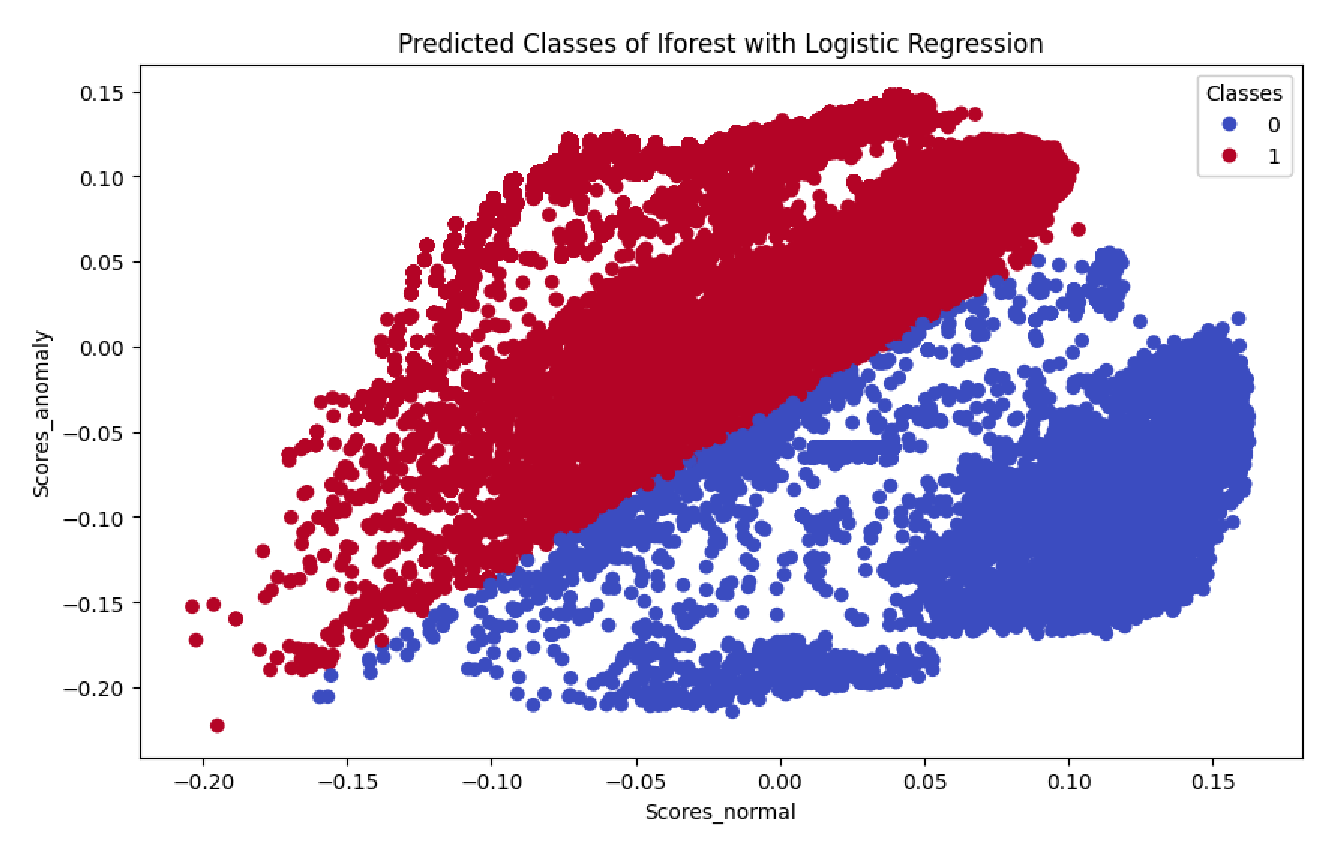
\includegraphics[width=\linewidth]{pictures/eps/UNSW1.eps}
    \caption{UNSW1(和文)}
    \ecaption{Description of the collectness\_UNSW figure (English).}
    \label{fig:UNSW1}
\end{figure}

\begin{figure}[tb]
    \centering
    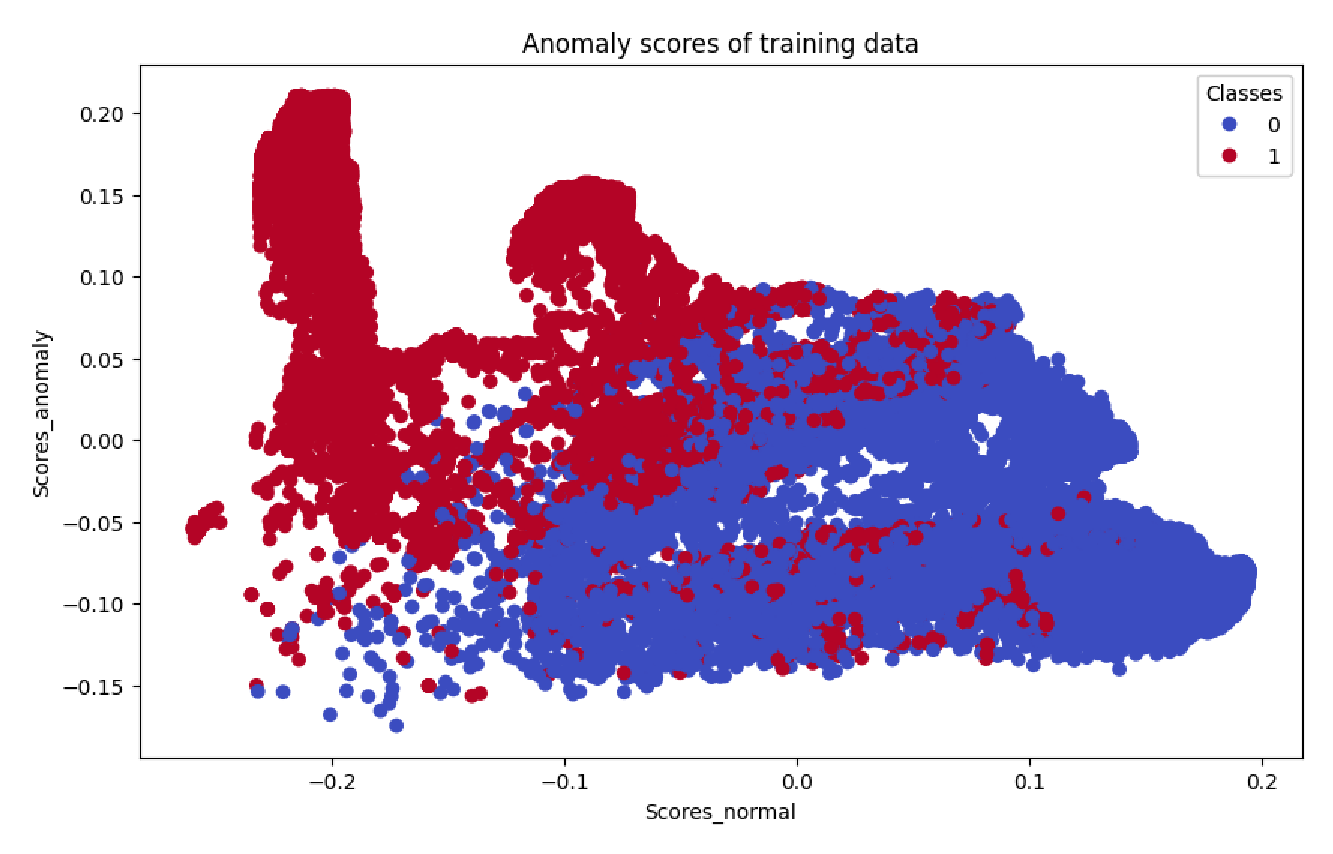
\includegraphics[width=\linewidth]{pictures/eps/NSL1.eps}
    \caption{NSL1(和文)}
    \ecaption{Description of the collectness\_UNSW figure (English).}
    \label{fig:NSL1}
\end{figure}

結果は以下の通りである。

\begin{table}[tb]
    \caption{UNSWでのモデルの性能評価結果(和文)}
    \ecaption{Performance evaluation results of models (English).}
    \centering
    \footnotesize
    \begin{tabular}{lcccc}
        \hline\hline
        model & accuracy & precision & recall & f1 \\
        \hline
        特徴量選択なし & 0.7506 & 0.7949 & 0.7506 & 0.7526 \\
        特徴量選択あり & 0.8440 & 0.9321 & 0.8440 & 0.8817 \\
        ロジスティック回帰で判定 & 0.9112 & 0.9146 & 0.9112 & 0.9082 \\
        \hline
    \end{tabular}
    \label{tab:model_performance}
\end{table}

\begin{table}[tb]
    \caption{NSLでのモデルの性能評価結果(和文)}
    \ecaption{Performance evaluation results of models (English).}
    \centering
    \footnotesize
    \begin{tabular}{lcccc}
        \hline\hline
        model & accuracy & precision & recall & f1 \\
        \hline
        特徴量選択なし & 0.7873 & 0.8749 & 0.7873 & 0.8171 \\
        特徴量選択あり & 0.8466 & 0.9174 & 0.8466 & 0.8775 \\
        ロジスティック回帰で判定 & 0.9452 & 0.9453 & 0.9452 & 0.9452 \\
        \hline
    \end{tabular}
    \label{tab:model_performance}
\end{table}

この結果から、2つのデータセットにおいて、特徴量選択を行うことで精度が向上することがわかった。また、ロジスティック回帰を用いて判定を行うことで、精度が向上することがわかった。



\begin{figure}[tb]
    \centering
    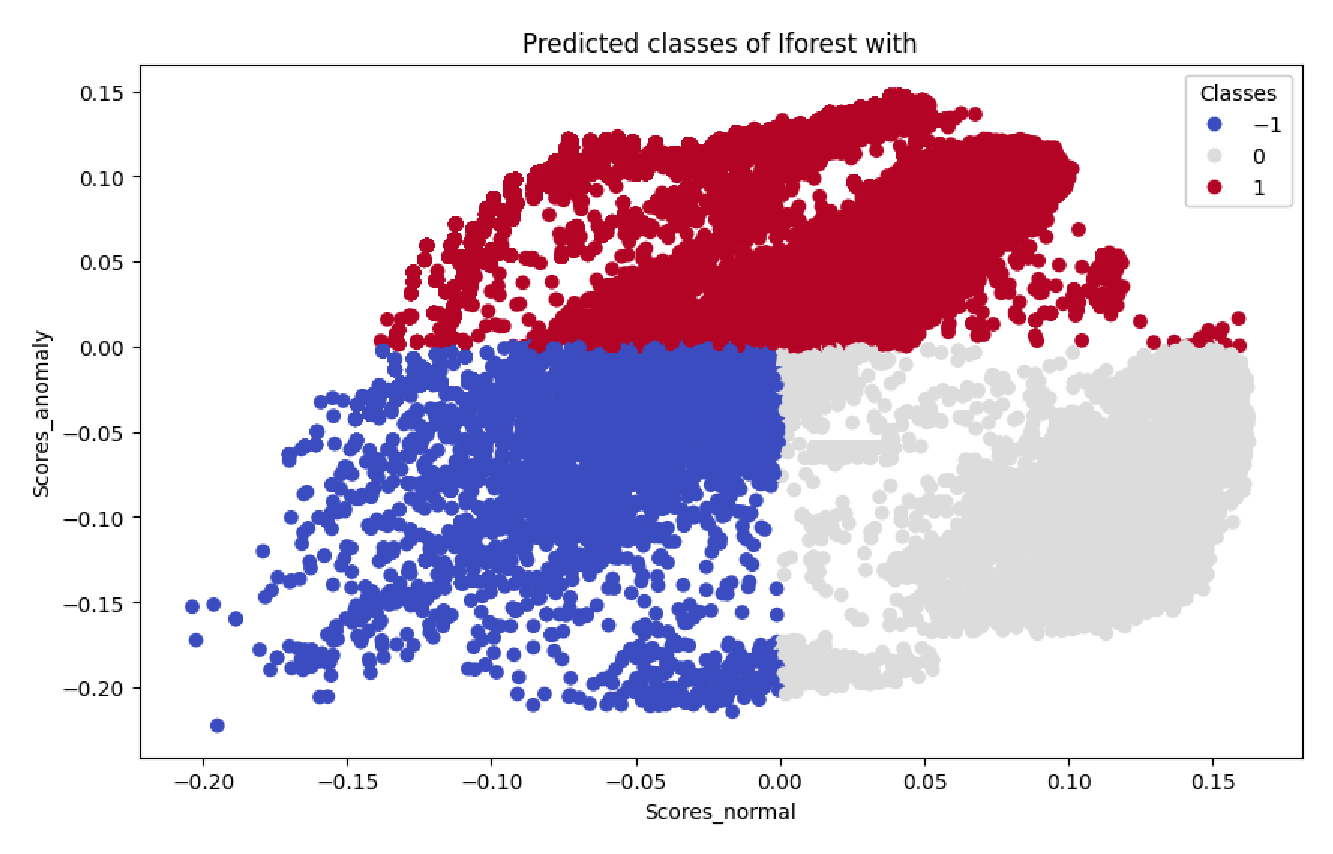
\includegraphics[width=\linewidth]{pictures/eps/UNSW2.eps}
    \caption{UNSW2(和文)}
    \ecaption{Description of the collectness\_UNSW figure (English).}
    \label{fig:UNSW2}
\end{figure}


\begin{figure}[tb]
    \centering
    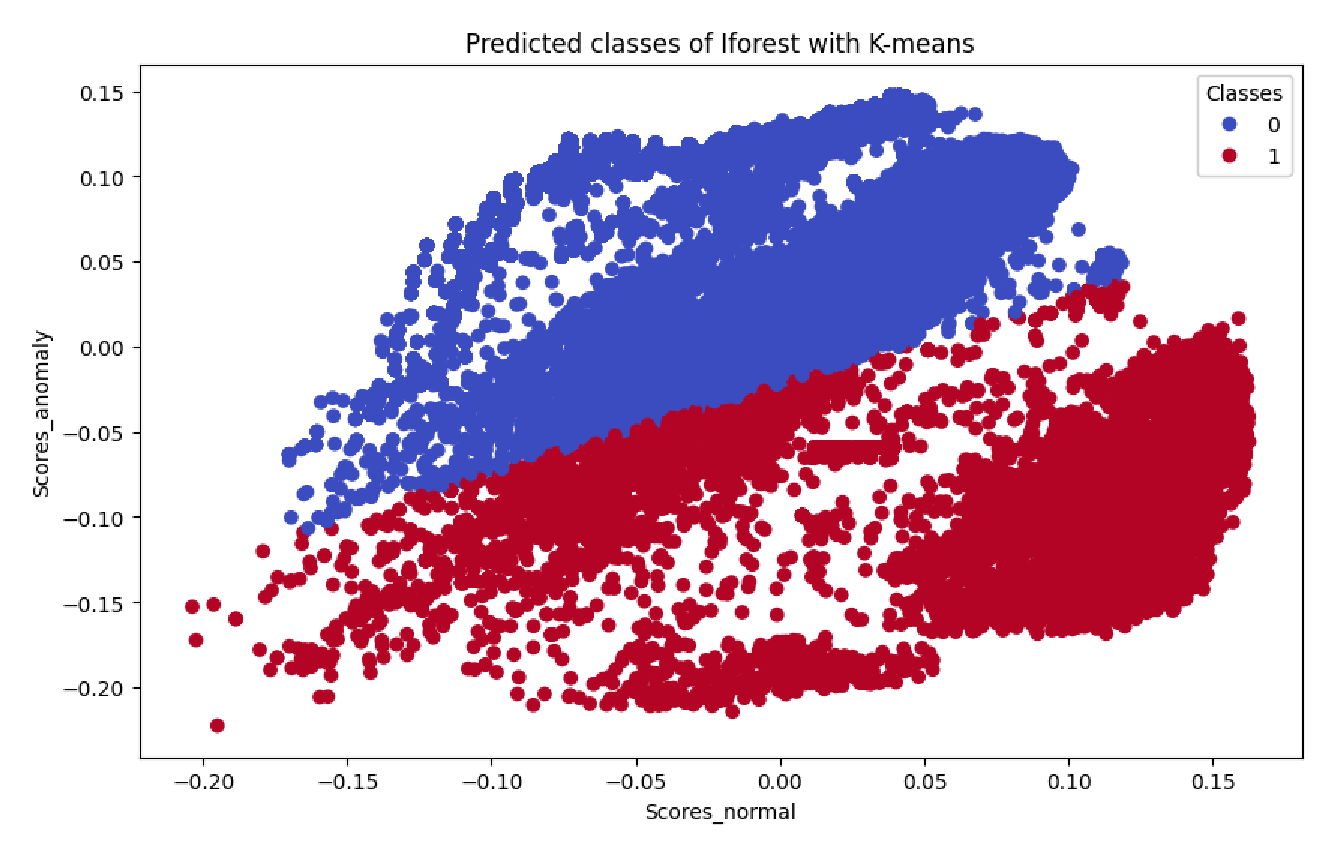
\includegraphics[width=\linewidth]{pictures/eps/UNSW3.eps}
    \caption{UNSW3(和文)}
    \ecaption{Description of the collectness\_UNSW figure (English).}
    \label{fig:UNSW3}
\end{figure}


\begin{figure}[tb]
    \centering
    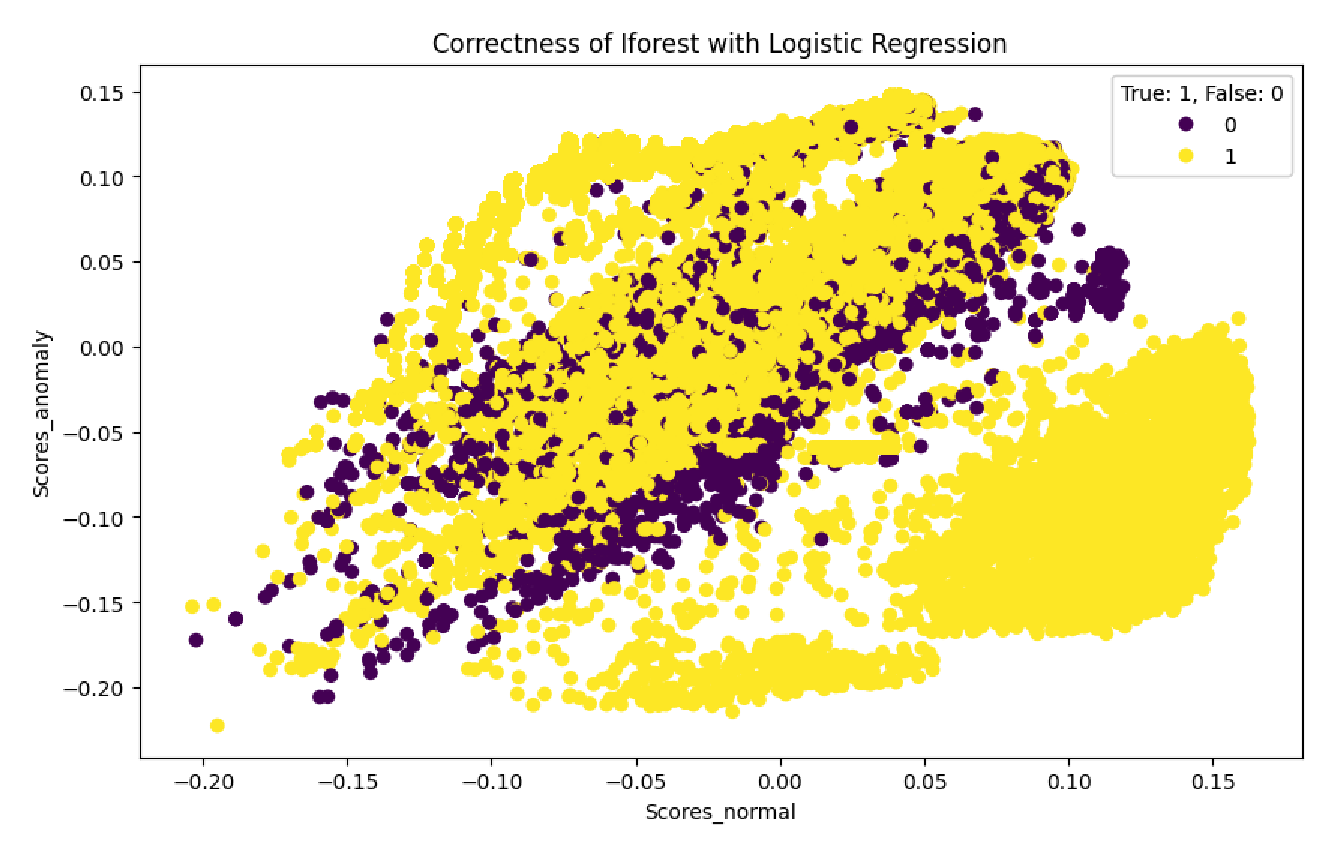
\includegraphics[width=\linewidth]{pictures/eps/UNSW4.eps}
    \caption{UNSW4(和文)}
    \ecaption{Description of the collectness\_UNSW figure (English).}
    \label{fig:UNSW4}
\end{figure}

\begin{figure}[tb]
    \centering
    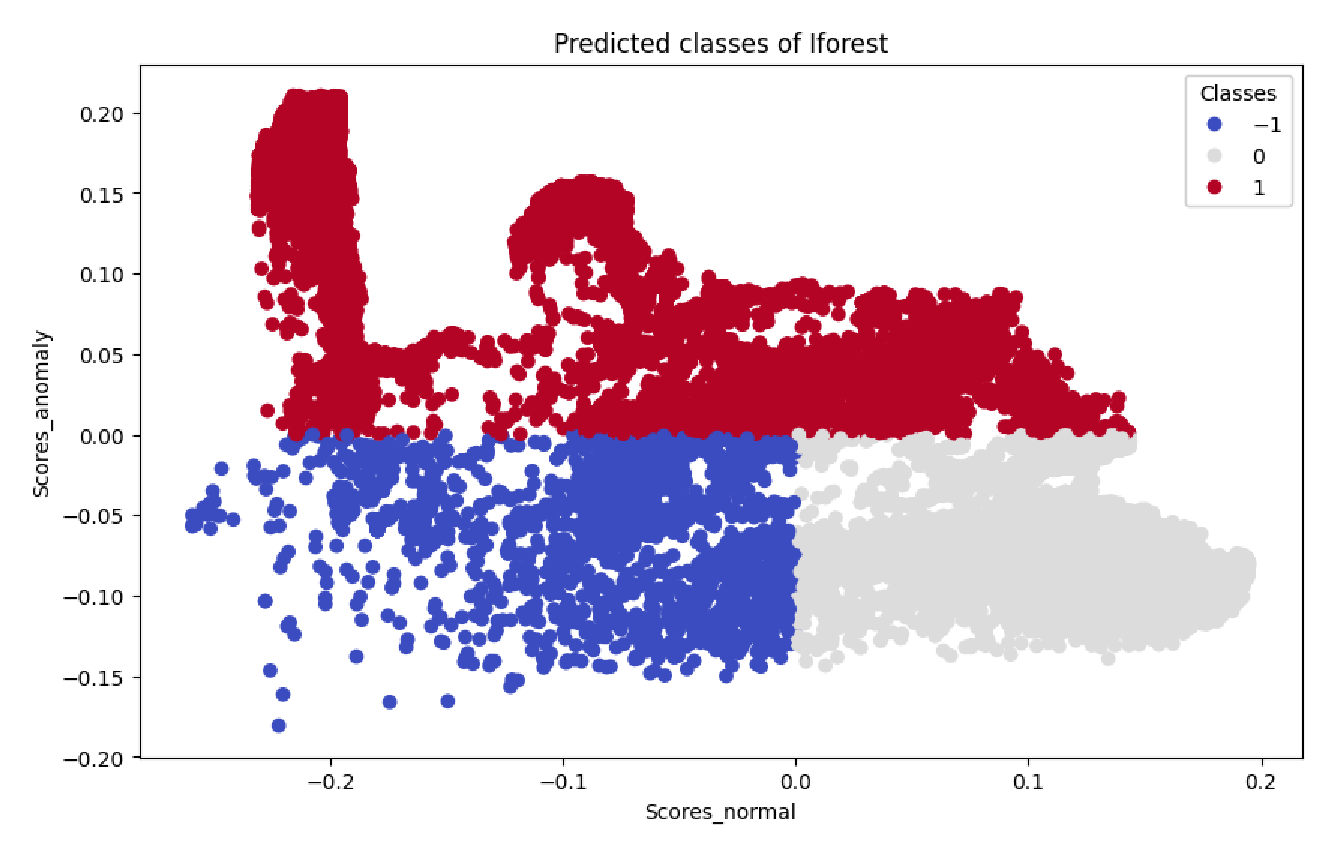
\includegraphics[width=\linewidth]{pictures/eps/NSL2.eps}
    \caption{NSL2(和文)}
    \ecaption{Description of the collectness\_UNSW figure (English).}
    \label{fig:NSL2}
\end{figure}

\begin{figure}[tb]
    \centering
    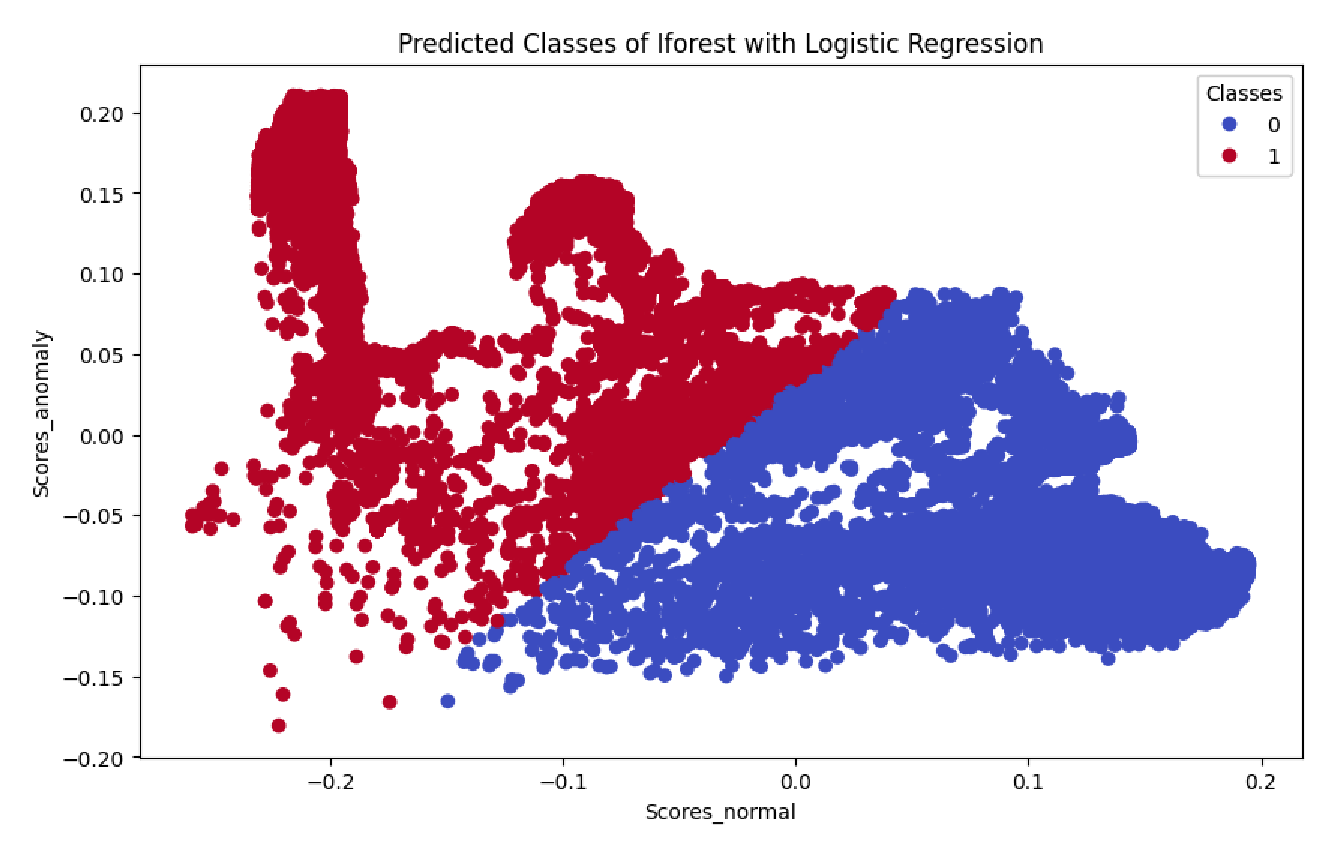
\includegraphics[width=\linewidth]{pictures/eps/NSL3.eps}
    \caption{NSL3(和文)}
    \ecaption{Description of the collectness\_UNSW figure (English).}
    \label{fig:NSL3}
\end{figure}

\begin{figure}[tb]
    \centering
    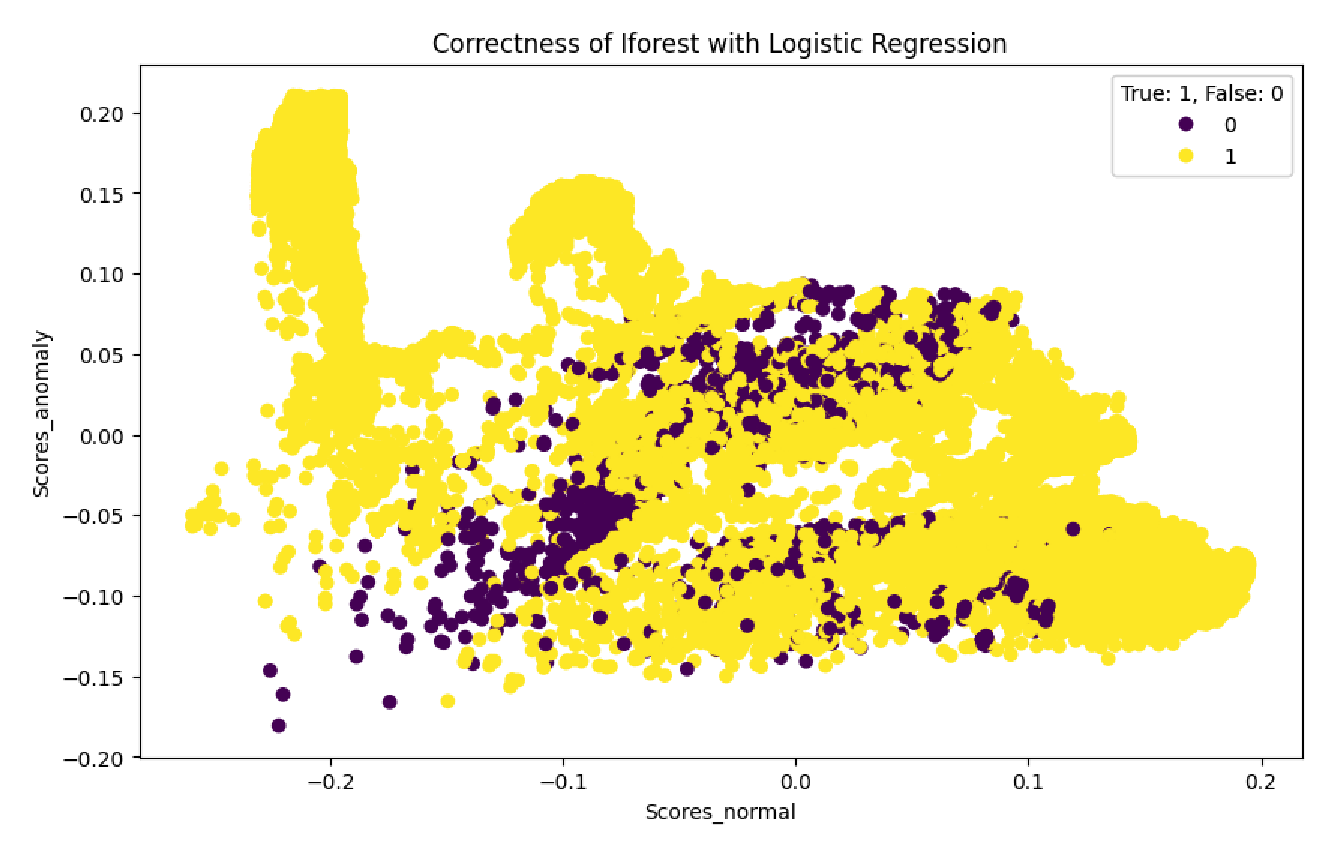
\includegraphics[width=\linewidth]{pictures/eps/NSL4.eps}
    \caption{NSL4(和文)}
    \ecaption{Description of the collectness\_UNSW figure (English).}
    \label{fig:NSL4}
\end{figure}

\subsection{考察}
今回の実験から、特徴量選択を行うことで精度が向上することがわかった。また、ロジスティック回帰を用いて判定を行うことでも精度が向上させられることがわかった。これは、今回使用した2つのデータセットの異常スコアの分布の境界線が斜めであり、線形な境界線でうまく分割できたためであると考えられる。
境界線が曲面であったり、データセットが

混ざってしまっている場合、うまくいかない
→なんでこれをiforesetを使っているのか
→判定の速さが

plusAlphaでかければいいこと
モデル構築のコストの比較
・ロジスティック回帰のコストvsiforestの探索()
の計算量(時間)を比較する

ロジスティック回帰におけるランダムサンプルしての精度の比較(調べてもいい)
サンプリングの適用範囲(データ量と精度のトレードオフ)

svcc 判定の決定技を作成して
(さまざまな観点から
決定技だとredteamと合意できる)
first(国際機関のcert)
≠≠≠≠


\section{おわりに}
おわりにを書く.

\begin{acknowledgment}
謝辞を書く.
\end{acknowledgment}

\begin{thebibliography}{10}

\end{thebibliography}

\end{document}
